\documentclass[11pt,a4paper]{article}

%% Language and font encodings
\usepackage[utf8]{inputenc}
\usepackage[margin=1in]{geometry}
\usepackage{authblk}
\usepackage[style=apa]{biblatex}
\usepackage[american]{babel}
\usepackage[finalizecache,cachedir=.]{minted}
\usepackage{csquotes}
\DeclareLanguageMapping{american}{american-apa}
\bibliography{references.bib}

\usepackage{amsmath,amsfonts,amssymb,bm,bbm,amsthm}
\usepackage[colorinlistoftodos,textsize=small]{todonotes}
\usepackage{graphicx}
%\usepackage{breqn}
\usepackage{todonotes}
\usepackage{xcolor} % color math symbols, delete later
\usepackage{verbatim}
\newcommand\todoin[2][]{\todo[inline, caption={2do}, #1]{
	\begin{minipage}{\textwidth-4pt}#2\end{minipage}}
}
\usepackage{nicefrac}

\theoremstyle{definition} % no italiced theorem style
\newtheorem{prop}{Proposition}
\newtheorem{corr}{Corollary}[prop]
\newtheorem{lemma}[prop]{Lemma}

\newtheoremstyle{case}{}{}{}{}{}{:}{ }{}
\theoremstyle{case}
\newtheorem{case}{Case}

\usepackage[colorinlistoftodos,textsize=small]{todonotes}
\usepackage[colorlinks=true, allcolors=blue, bookmarks=false]{hyperref}


\newcommand{\iu}{{i\mkern1mu}}
\newcommand{\Lik}{\mathbb{L}}
\newcommand{\bx}{\bm{x}}
\newcommand{\by}{\bm{y}}
\newcommand{\bz}{\bm{z}}
\newcommand{\Reals}{\mathbb{R}}
\newcommand{\dx}[1]{\enspace \mathrm{d}{#1}}
\newcommand{\prior}[1]{\pi\left({#1}\right)}
\newcommand{\FGamma}[1]{\Gamma\left({#1}\right)}
\newcommand{\FBeta}[2]{\text{B}\left({#1},\ {#2}\right)}
\newcommand{\FHyperG}[1]{\, _2F_1\left({#1}\right)}
\newcommand{\FHyperGn}{\, _2F_1}
\newcommand{\mean}[1]{\overline{{#1}}}
\newcommand{\Lim}[1]{\raisebox{0.5ex}{\scalebox{0.8}{$\displaystyle \lim_{#1}\;$}}}
\newcommand{\BF}{\text{BF}}
\newcommand{\FHypGeo}[4]{\,_2F_1\left({#1};{#2};{#3};{#4}\right)}
\newcommand{\BetaBinom}[4]{\text{BB}\left(#1 \mid #2 ,\ #3 ,\ #4 \right)}

\newcommand{\dist}[1]{\pi\left(#1\right)}
\newcommand{\scaledDirichlet}[3]{\text{SD}\left(#1 \mid #2 ,\ #3\right)}
\newcommand{\simplex}[1]{\mathbb{S}^{#1}}
\newcommand{\Expectation}[1]{E\left[#1\right]}

\DeclareRobustCommand{\stirling}{\genfrac\{\}{0pt}{}}
\newcommand{\rstirling}[3]{\stirling{#1}{#2}_{#3}}
\newcommand{\bellnum}[1]{B_{#1}}
\newcommand{\rbellnum}[2]{B_{#1,\,#2}}

\newcommand*\samethanks[1][\value{footnote}]{\footnotemark[#1]}

\newcommand{\numberthis}{\addtocounter{equation}{1}\tag{\theequation}}
\newcommand{\FD}[1]{\todo[inline, color=pink]{ \textbf{FD}: #1 }}
\newcommand{\DB}[1]{\todo[inline, color=orange]{ \textbf{DB}: #1 }}

\date{}
\title{Flexible Bayesian Multiple Comparison Adjustment}
\author[1]{Don van den Bergh\thanks{These authors contributed equally to this work.}}
\author[1]{Fabian Dablander\samethanks[1]}
\author[1]{Eric-Jan Wagenmakers}
\affil[1]{Department of Psychological Methods, University of Amsterdam}


\begin{document}
\maketitle

\section*{Outline}
\begin{enumerate}
    \item Introduction / Motivation
    \begin{itemize}
        \item Multiplicity adjustment for multiple comparisons
        \item Testing all possible hypotheses in an automatic manner (compared to frequentist setting, where this is not easy ... one would have to do this manually, which completely screws up multiple comparison procedures (I think!)): could sort the means and do $K - 1$ comparisons; errors might get exacerbated (one error early on puts lots of means into wrong partition); Rao's paradox (not reject the pairwise comparisons but would reject the joint); score-based likelihood approach (but computational explosion; K = 12 equals $>$ 4 million comparisons)
        \item Clustering of group-level parameters (in what sense is the DPP applied to the ANOVA setting equivalent to an infinite Gaussian mixture model?)
        \item DP as a motivation to penalize multiplicity but also as a feasible way to do computations on the space of all partitions
    \end{itemize}
    \item Methodology
    \begin{itemize}
        \item Prior over all partitions, refer to Dirichlet Process Prior \parencite{gopalan1998bayesian}
        \item Introduce the beta-binomial prior for this purpose \parencite{scott2006exploration}
        \item Quantify the degree of multiplicity adjustment for pairwise comparisons by extending the trick in \textcite{scott2010bayes} and \textcite{li2016role}
        \begin{itemize}
            \item Either compute $\frac{P(\mu_i = \mu_j | K)}{P(\mu_i = \mu_j | K + 1)}$ where $K$ indexes the number of groups; or compute the ratio of the probability that an additional group is equal to one of the other groups or not. Plot this ratio quantity as a function of the number of groups.
            \item Intuitively, as the number of groups grow, this ratio should grow as well (the new group mean is more likely to be equal to already observed group means). It is this shrinkage what gives multiplicity control.
            \item \textcite{scott2010bayes} study multiplicity adjustment by adding a bunch of variables that have zero effect and looking at how the posterior inclusion probabilities change. What would be the analogue for our multiple comparison case? Adding group means that are all equal?
            \item NB: the problem of multiplicity seems worse in variable selection; while there are more (pairwise) comparisons possible in ANOVA settings, one comparison gives information about all other comparisons involving that group.
        \end{itemize}
        \item Could we use variational inference to speed up computations? Probably tough to get it to converge
        \item Need to look into the consistency of the DP estimate \parencite[e.g.,][]{diaconis1986consistency, ghosal2017fundamentals}
        \item Another motivation of the prior is to look at the expected number of clusters for $n$ observations. For the Dirichlet process prior, one can show \parencite[e.g.,][]{teh2010dirichlet} that the expected number of clusters frrom $n$ observations is approximately given by $\alpha \text{log}\left(1 + \frac{n}{\alpha}\right)$. Would be insightful to derive a similar formulate for the beta-binomial prior.
        \item Beta-binomial does distinguish the greens from the oranges qua frequency; compare with Dirichlet process prior
        \item \textcolor{red}{New remarks: Do the priors we use introduce an exchangeable series for $\theta$? How are the expected cluster sizes related to the partitions? It's 1:1, because clusters are partitions in our case.}
    \end{itemize}
    \item Applications
    \begin{itemize}
        \item Proportions
        \item One-way ANOVA
        \item Variances
    \end{itemize}
    \item Conclusion
\end{enumerate}

\section{Introduction}
Assessing the equality or inequality of groups is a key problem in science and applied settings. In experimental psychology, for example, memory researchers study whether a set of learning techniques differ in ... (CITE). In marketing, companies are interested in assessing the effect of distinct interventions (CITE). In political science, researchers ...

If a confirmatory hypothesis is lacking, a standard approach is to first test whether all groups are equal, and if not, engage in multiple post-hoc comparisons. A large swathe of multiple comparisons techniques to guard against inflated false positive errors exist in classical statistics dating back to the work of John Tukey and others \parencite[][]{rao2009multiple, benjamini2002john}. From a Bayesian perspective, the problem of multiple comparisons can be addressed by changing the model prior \parencite{jeffreys1961theory, westfall1997bayesian, berry1999bayesian}, which has found prominent application in variable selection for regression \parencite[e.g.,][]{scott2006exploration, scott2010bayes}. Here, we focus on a Bayesian multiplicity adjustment for testing the (in)equality of a set of groups by proposing a prior distribution over all possible partitions. This allows the researcher to explore the set of all possible equality and inequality relations among the groups while penalizing for multiple comparisons, a feat that is difficult to solve in a principled manner in classical statistics.

The paper is structured as follows. In Section 1, we briefly review the Bayesian literature on multiple comparison and specify the setup. In Section 2, we describe the Polya urn scheme from which a number of priors can be derived that account for multiplicity. We focus on four such priors in Section 3, and present a simulation study comparing them. In Section 4, we illustrate our method on practical examples related to the comparison of means, variances, and proportions. Our method is available in the Julia package \textit{EqualitySelection}.


\section{Problem Setup}
Our goal is to adjust for multiple comparisons in a flexible manner. Multiple comparisons are not a problem if a researcher wishes to compare only two hypothesis, denote them as $\mathcal{H}_0$ and $\mathcal{H}_1$. They way to do this is through use of the Bayes factor \parencite[e.g.,][]{kass1995bayes, ly2016harold}, which is given by:

\begin{equation}
    BF_{10} \equiv \frac{p(\mathcal{D} \mid \mathcal{H}_1)}{p(\mathcal{D} \mid \mathcal{H}_0)} \enspace ,
\end{equation}

where $\mathcal{D} = (Y_1, \ldots, Y_n)$ is the data. The Bayes factor does not depend on the number of hypotheses a researcher wishes to test. It is the same regardless of whether the researcher, say, is a neuroscientist and tests whether there is activity in one voxel or in $10,000$. A principled way to account for multiplicity is by adjusting the prior probability of the hypotheses \parencite[e.g.,][]{jeffreys1961theory, westfall1997bayesian}.

Suppose the researcher is interested in comparing $K$ groups, parameterized by $\theta = (\theta_1, \ldots, \theta_K)$. She is not only interested in whether all parameters are equal ($\mathcal{H}_0$) or whether they are unequal ($\mathcal{H}_1$), but also which pairs of parameters are equal or not. In the language of classical statistics, she is interested in post-hoc comparisons. We focus on a Bayesian solution to this problem in this paper. More specifically, going beyond classical tests, we consider the problem of assessing all possible equalities and inequalities between the groups. In general terms, the inference problem is:
\begin{align*}
    \theta &\sim \pi_{\theta}(.) \\
    \phi &\sim \pi_{\phi}(.) \\
    Y_i &\overset{i.i.d.}{\sim} P(Y_i \mid \theta, \phi)  \enspace ,
\end{align*}
where $\phi$ are nuisance parameters (in case they exist), such as the variances in an ANOVA, and $P$ is the likelihood. Using the posterior distribution of $\theta$, we can restate $\mathcal{H}_0$ as $p(\theta_1 = \theta_2 = \ldots = \theta_K \mid \mathcal{D})$ and $\mathcal{H}_1$ as $p(\theta_1 \neq \theta_2 \neq \ldots \neq \theta_K \mid \mathcal{D})$, but there are many more possible hypotheses, depending on the combination of equalities and inequalities. In the next section, we discuss and compare priors $\pi_{\theta}$ that allow for flexible multiplicity adjustment.


\section{Methodology}
% I think it makes sense to first explain why we use partitions

\subsection{Partitions}
The space of possible equality constraints for some parameter vector $\mathbf{\theta} = (\theta_1, \ldots, \theta_k)$ of size $k$ is equivalent to the partitions of that vector. For example, if $k = 3$ then the model that states $\theta_1 = \theta_2 \neq \theta_3$ is equivalent to the partition $\{\{\theta_1, \theta_2\}, \{\theta_3\}\}$. The space of possible models for $k = 4$ is shown in Figure~\ref{fig:partitions}.

\begin{figure}
    \centering
    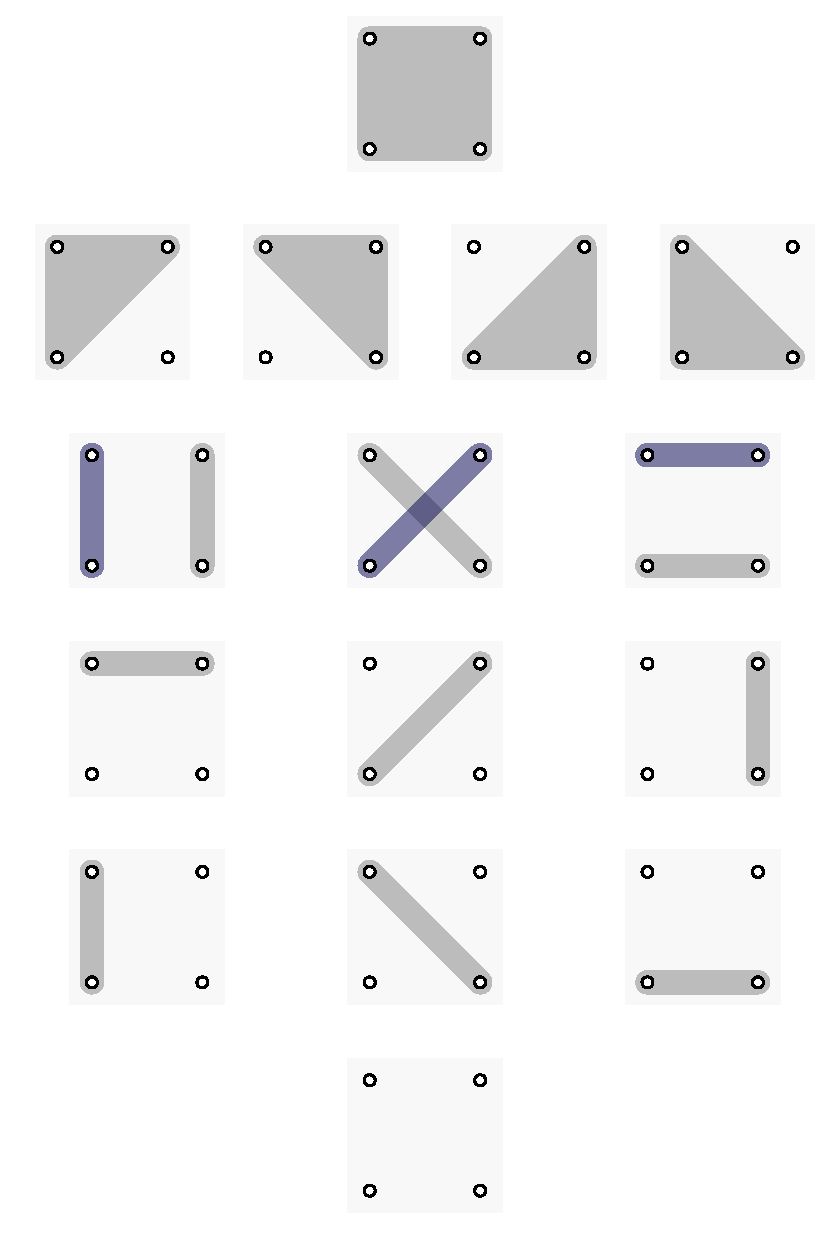
\includegraphics[width = \textwidth, keepaspectratio]{figures/modelspace_4_vertical.pdf}
    \caption{All possible models given $k = 4$, represented as partitions. Circles represent individual parameters and shaded regions indicate which parameters are equal.}
    \label{fig:partitions}
\end{figure}
\DB{Do we want to follow APA7?}

This equivalence is useful as partitions have been studied extensively in combinatorics. Given $k$ parameters, the number of partitions of size $j$ is given by the Stirling numbers of the second kind, denoted $\stirling{k}{j}$. The total number of partitions is given by the $k$\textsuperscript{th}-Bell number, which is defined as a sum over the Stirling numbers:
\begin{equation}
    \bellnum{k} = \sum_{i = 0}^k \stirling{k}{j} \enspace .
\end{equation}
The Bell numbers grow very quickly, with the number of partitions for a vector $\mathbf{\theta}$ of size 10 being $B_{10} =115975$. % B_10, not B_9 (21147)

The Stirling numbers and Bell numbers can be generalized to the $r$-Stirling \parencite{broder1984r} and $r$-Bell numbers \parencite{mezo2011r}. These generalizations help to construct conditional distributions, as will be shown later. The $r$-Stirling numbers $\rstirling{k}{j}{r}$ give the number of partitions of size $j$ given a $k$ parameters such that the first $r$ parameters are all in distinct subsets. The $r$-Bell numbers give the total number of partitions given $k$ parameters where the first $r$ parameters are in distinct subsets. Specifically, we have
\begin{align}
    \rstirling{k}{j}{r} &= \sum_{i=0}^k \binom{k}{i}\stirling{i}{j}r^{k-i}\\
    \rbellnum{k}{r} &= \sum_{i=0}^k \rstirling{k+r}{i+r}{r} \enspace .
\end{align}
Note that $\rstirling{k}{j}{1} = \stirling{k}{j}$ and that $\rbellnum{k}{0} = \bellnum{k}$. Both the $r$-Stirling and $r$-Bell are defined through recurrence relations, although explicit expressions exist which are easier to compute for large values. See \textcite{broder1984r} and \textcite{mezo2011r} for details.

\subsection{Urn Schemes}
Statistically, we represent the different partitions using an urn with $K$ different balls labeled 1 through $K$. For each parameter $\theta_i$, a ball $b_i$ is drawn from the urn with $b_i \in \{1,K\}$. If two drawn balls are equal, $b_i = b_j$, then the two parameters are assigned to the same subset of the partition, i.e., the two parameters, $\theta_i$ and $\theta_j$, are equal if $b_i = b_j$. Note that different draws from an urn can represent the same partition. For example, the draws $(1, 1, 2)$ and $(3, 3, 1)$ both represent the partition $\{\{\theta_1, \theta_2\}, \{\theta_3\}\}$. The prior distributions introduced in the next sections assign probabilities to the unique partitions. The prior probability for a particular draw can be obtained by dividing the probability of the corresponding partition by the total number of draws that correspond to that partition. The total number of draws that represent the same partition is given by $d!\binom{k}{d}$ where $d$ is the number of non-empty subsets of a particular draw. 

% not sure how to bring this up
Although the urn consists of $K$ different balls, the event of interest is the whether the next ball drawn equals one of the balls already drawn. In other words, whether an equality or inequality is introduced. This event reduces the urn to a P\'{o}lya urn. All prior distributions discussed below are related to the P\'{o}lya urn.

Specifically, the joint prior distribution on $(\theta_1, \ldots, \theta_K)$ is characterized by a (generalized) P\'{o}lya urn such that:

\begin{equation} \label{eq:prediction-rule}
    P(\theta_i \mid \theta_1, \ldots, \theta_{i - 1}) = \begin{cases}
    \zeta_i & \text{with probability } P_{\pi} \\
    \theta_i^{\star} & \text{with probability }  1- P_{\pi} \enspace ,
    \end{cases} \numberthis
\end{equation}

where $\zeta_i$ denotes a new value for $\theta_i$ and $\theta_1 = \zeta_1$; and $\theta_i^{\star}$ denotes a value equal to any previously observed value. We characterize the priors we discuss in the next section in terms of (\ref{eq:prediction-rule}), which is known as a \textit{prediction rule} \parencite[e.g.,][]{ishwaran2001gibbs}; in terms of the expected number of clusters; and, most importantly, in terms of their penalty for multiplicity.

\FD{\textcite{ishwaran2001gibbs} might be useful, they use Polya Urns to derive a Gibbs sampler. They say it can be used for the Dirichlet process, but also for \textit{any} prior with known \textit{prediction rule}, which is defined as $P(Y_{n+1} \mid Y_1, \ldots, Y_n)$. I think this is a useful description which allows us to distinguish between several priors (Dirichlet, Pittman-Yor, Beta-binomial, etc.). Maybe note this here and then we refer to the next sections, in which we discuss the priors in slightly more detail?}
% We want to make inference over all possible partitions of some population parameter vector $\mathbf{\theta} = (\theta_1, \ldots, \theta_k)$ of size $k$. Each such partition corresponds do one particular hypothesis. The number of partitions $k$ is given by the Bell number

% \begin{equation}
%     B_{k + 1} = \sum_{i = 0}^k {k \choose i} B_k \enspace .
% \end{equation}

% The Bell numbers grow very quickly, with the number of partitions for a vector $\mathbf{\theta}$ of size 10 being 21147.

\begin{itemize}
    \item \textcolor{red}{NEED A PLOT THAT SHOWS THE PARTITIONS NICELY}
\end{itemize}

\subsection{Pitman-Yor Process}
Let $(\theta^{\star}_{1, i}, \ldots, \theta^{\star}_{m_i, i})$ be the unique set of values in $(\theta_1, \ldots, \theta_{i-1})$, each occuring with frequency $n^{\star}_{j, i}$ for $j = \{1, \ldots, m_i\}$. The Pitman-Yor process $\mathcal{PY}(a, b)$ has a prediction rule given by:

\begin{equation}
    P(\theta_K \mid \theta_1, \ldots, \theta_{K - 1}) = \frac{b + a m_K}{b + K - 1} \mathcal{G}_0 + \sum^{m_K}_{j = 1} \frac{n^{\star}_{j, K} - a}{b + K - 1} \delta_{\theta^{\star}_{j, K}}(.) \enspace ,
\end{equation}

where $\mathcal{G}_0$ is the base distribution \parencite{ishwaran2001gibbs, pitman1997two}.

Let $m$ be the number of clusters among $K$ groups. Under the Pitman-Yor process, we have that as $K \rightarrow \infty$, the expected number of unique clusters $m$ in a partition is given by \parencite[e.g.,][]{wallach2010alternative}:

\begin{equation}
    \mathbb{E}[m \mid K] \approx \frac{\Gamma\left(1 + b\right)}{a\Gamma\left(a + b\right)}K^a \enspace .
\end{equation}

\FD{Are these asymptotic results useful for our max $K = 15$ setting? It seems that it might make more sense to calculate them exactly through simulations.}

\FD{\textcite{wallach2010alternative} show what the priors imply (asymptotically) in terms of the expected number of clusters of size $M$. So basically, what we force to be a Beta-binomial in our prior. I think it makes again sense to contrast this for the PY and the DP --- computed exactly through simulation --- with out beta-binomial.}

\subsection{Dirichlet Process Prior}
The Dirichlet Process prior is a Pitman-Yor process with $a = 0$ and $b = \alpha$, that is, $\mathcal{PY}(0, \alpha)$. The prediction rule is given by \parencite[e.g.,][]{ishwaran2001gibbs, blackwell1973ferguson}:

\begin{equation}
    P(\theta_K \mid \theta_1, \ldots, \theta_{K - 1}) = \frac{\alpha}{\alpha + K - 1} \mathcal{G}_0 + \sum^{m_K}_{j = 1} \frac{n^{\star}_{j, K}}{\alpha + K - 1} \delta_{\theta^{\star}_{j, K}}(.) \enspace .
\end{equation}.

Under the Dirichlet Process prior, we have that, as $K \rightarrow \infty$, the expected number of unique clusters $m$ in a partition is given by:
\begin{equation}
    \mathbb{E}[m \mid K] \approx \alpha \text{log}\left(1 + \frac{K}{\alpha}\right) \enspace ,
\end{equation}
see for example \textcite[][p. 8]{teh2010dirichlet}.
\FD{This seems to ignore that we learn about $\theta$ through observations $\mathcal{D}$ by means of a likelihood ... or not?}



\color{red}
\subsection{Dirichlet Process Prior}
\textcite{gopalan1998bayesian} suggest a Dirichlet process (DP) prior for this problem. A DP is a prior over probability distributions, first developed by \textcite{ferguson1973bayesian}. Let $H$ be a base distribution over a parameters $\Theta$ and $A_1, \ldots, A_r$ be a finite partition of $\Theta$. We have that if $G \sim DP(\alpha, H)$ then

\begin{equation}
    G(A_1), \ldots, G(A_r) \sim \text{Dir}(\alpha H(A_1), \ldots, \alpha H(A_r)) \enspace .
\end{equation}

In other words, a random distribution $G$ follows a Dirichlet process when its marginal distribution is a Dirichlet distribution. Let $(\theta_1, \ldots, \theta_n)$ be $n$ draws from $G$, and define $(\theta^{\star}_1, \ldots, \theta^{\star}_k)$ as the unique values of $(\theta_1, \ldots, \theta_n)$ and $n_j$ as the number of repeats of $\theta^{\star}_j$. Then

\begin{equation}
    G \mid \theta_1, \ldots, \theta_n \sim DP\left(\alpha + n, \frac{\alpha}{\alpha + n}H + \frac{1}{\alpha + n} \sum_{j=1}^k n_j \delta_{\theta^{\star}_j}\right) \enspace ,
\end{equation}

that is, the posterior of $G$ is another Dirichlet process. Suppose we observe a new population parameter $\theta_{n + 1}$. We have that:

\begin{equation}
    \theta_{n + 1} \mid \theta_1, \ldots, \theta_n \sim \frac{1}{\alpha + n} \left(\alpha H + \sum_{j=1}^k n_j \delta_{\theta^{\star}_j}\right) \enspace .
\end{equation}

In other words, the probability that $\theta_{n + 1}$ takes a new value is proportional to $\nicefrac{\alpha}{\alpha + n}$, and the probability that it equals one of the already observed population parameters is proportional to $\nicefrac{n}{\alpha + n}$; in particular, it is drawn proportional to the number of already observed values $\theta^{\star}_j$, $n_j$.

The unique values of $(\theta_1, \ldots, \theta_n)$ induce a partitioning of the set $[n] = \{1, \ldots, n\}$ into clusters $(\theta^{\star}_1, \ldots, \theta^{\star}_k)$ such that, within each cluster $j$, we find $n_j$ number of $\theta_i$'s with value $\theta^{\star}_j$. This distribution over partitions is known as the \textit{Chinese Restaurant Process}.

In the settings we consider, $\mathbf{\theta}$ is a population parameter vector which we infer from data. \textcite{antoniak1974mixtures} showed that the posterior over $G$ is a mixture of Dirichlet processes when we learn about $\theta$ not directly but through data.
\color{black}

\subsection{Uniform Prior}
\FD{The paper by \textcite{wallach2010alternative} seems extremely relevant here. The define the uniform process as having a prediction rule that is uniform over the already existing partitions ... so not quite the same. How is it related to what we do here? Actually, they show that the expected number of clusters of size $M$ is a constant, so it seems to be exactly what we do. Interestingly, the uniform process is not exchangeable. Also, it seems to me that it will not penalize multiplicity.}
For completion, we derive a prior that is uniform over the space of partitions. The probability mass function is straightforward. All valid configurations of size $k$ have probability $1 / \bellnum{k}$.
\DB{I could give the conditional distributions here, as well as the prior probability of equating $j$ out of $k$ parameters. That could then come back at the Beta-Binomial part. Do we want that though?}

\subsection{Beta-Binomial Prior}
Here we briefly introduce the Beta-Binomial model prior, its properties, and how we can apply use it to the space of equality constraints. The Beta-Binomial model prior is often-used in linear regression when doing stochastic search variable selection \parencite[SSVS;][]{george1993variable} or Bayesian Model Averaging \parencite[BMA;][]{hinne2020conceptual, hoeting1999bayesian}. It states that the prior probability of including $j$ predictors out of a total of $k$ predictions is given by
\begin{equation}
    \BetaBinom{j}{k}{\alpha}{\beta} = \binom{k}{j} \frac{\FBeta{j + \alpha}{k - j + \beta}}{\FBeta{\alpha}{\beta}} \enspace ,
\end{equation}
where $\alpha$ and $\beta$ are hyperparameters. The prior probability of a particular model is obtained by dividing by the number of ways $j$ out of $k$ predictors can be included: $\BetaBinom{j}{k}{\alpha}{\beta} / \binom{k}{j}$. The advantage of the Beta-Binomial distribution is that it introduce a penalty for including additional predictors and in that way introduces a correction for multiplicity \parencite{scott2010bayes}.

In the space of equality constraints, we consider the number of inequality constraints and use the Beta-Binomial prior to introduce a penalty for each additional inequality among the variables considered. This yields the following prior distribution over the number of included inequalities: $\BetaBinom{j}{k-1}{\alpha}{\beta}$. To obtain the prior probability for a particular model, divide by the number of ways we can choose $j$ out of $k-1$ inequalities and obtain $\BetaBinom{j}{k-1}{\alpha}{\beta} / \stirling{k}{k-j}$.


\begin{itemize}
    \item \textcolor{red}{NEED A PLOT THAT SHOWS PRIOR OVER PARTITIONS + INCLUSION PROBABILITIES FOR UNIFORM AND BETA-BINOMIAL}
\end{itemize}

\subsection{Comparison of Priors}

\begin{itemize}
    \item \textcolor{red}{NEED SCOTT \& BERGER PLOT FOR THE THREE PRIORS}
    \item \textcolor{red}{NEED A PLOT SHOWING THE EXPECTED NUMBER OF CLUSTERS}
\end{itemize}



\section{Simulation Study}

\section{Discussion}
\textcite{kim2009spiked} combine a spike at zero with a DPP. \textcite{curtis2011bayesian} also use a DPP to combine clustering o highly correlated predictors in linear regression with variable selection. \textcite{canale2017pitman} focus on the Pitman-Yor process, which is a generalization of the DPP. \textcite{lu2018reducing} study a powered Chinese restaurant process. \textcite{miller2015microclustering} study a microclustering property, for which the number of data points in a cluster does not grow linearly with the total number of data points (which is assumed by the DP, PY, etc.)

%\textit{This paper grew out of our response to an anonymous reviewer of another paper.}

\printbibliography
\end{document}